

The manipulations of MPO's is done by manipulating the tensor into a matrix, performing some matrix calculations and casting it back into it's original form. This section gives some examples how these manipulations are done in practice:

\subsection{decomposition} \label{decompMPO}

\def \figone {\expH{2}{$O^{u v,v w}$}{{"$i_1$","$i_2$"}}{{"$j_1$","$j_1$"}}{{"u","w"}}}


\begin{equation}
    \begin{split}
        \figone &= O^{i_1 i_2 j_1 j_2 }_{\alpha_u \gamma_w} \\
        &\cong O^{u w}_{ (\alpha_u i_1 j_1) (\gamma_w i_2 j_2) } \\
        &= O^{u v}_{(\alpha_u i_1 j_1) \beta_v } O^{v w}_{ \beta_v (\gamma_w i_2 j_2) } \\
        &\cong \mpo{2}{{"u","v","w"}}{{"$i_1$","$i_2$"}}{{"$j_1$","$j_1$"}}{}{}
    \end{split}
\end{equation}

Step 2 reshapes and groups the indices to one index. The dimension of this index is the sum of the seperate dimensions. Step 3 decomposes the matrix into a product of 2 matrices. The last step transforms the indices back to separate legs.

For an exact representation, the bond dimension of virtual level v is:
\begin{equation}
    \dim{v} = \min( \dim{u}, \dim{v}) + 2 \dim{i}
\end{equation}


Many different matrix decompositions exist. Some usefull examples here are svd decomposition and eigenvalue decomposition. The split in left and right matrix is not unique and differs per algoritm.


\subsection{inverse}
Suppose we want to find a MPO O for given tensors A and B such that the following holds:

\def \figone {\expH{2}{$A$}{{"$i_1$","$i_2$"}}{{"$j_1$","$j_2$"}}{{"u",}}}
\def \figthree {\expH{3}{$B$}{{"$i_1$","$i_2$","$i_3$"}}{{"$j_1$","$j_2$","$j_3$"}}{{"u","v"}}}

\def \figtwo {\mpo{1}{{,"v"}}{{"$i_3$",}}{{"$j_3$",}}{}{}}

\begin{equation}
    \combineTikz{ \figone }{\figtwo}{1.8} =  \figthree
\end{equation}

Again, the indices can be taken toghether in the following way: $\alpha = (u i_1 j_1  i_2 j_2)$ and $\beta = (i_3 j_3 v)$:
\begin{equation}
    A_{\alpha \gamma} O_{\gamma \beta} = B_{\alpha \beta}
\end{equation}
This a a standard matrix equation and can hence be solved with linear algebra packages. Note that it is not necessary to calculate $A^{-1}$ to obtain the solution. In matlab the procedures mldivide and lsqminnorm can be used, which give more robust solutions.

The solution will be denoted by

\def \figoneb {\expH{2}{$A$}{{,}}{{,}}{{,"w"}}}
\def \figonec {\expH{2}{$A^{-1}$}{{,}}{{,}}{{"w",}}}
\def \figthreeb {\expH{3}{$B$}{{,,"$i_3$"}}{{,,"$j_3$"}}{{,"v"}}}

\def \figtwob {\mpo{1}{{"w","v"}}{{"$i_3$",}}{{"$j_3$",}}{} {}}

\def \figfour { \expH{1}{$A^{-1}B$}{{"$i_3$",}}{{"$j_3$",}}{{"u","v"}} }

\begin{equation}
    \begin{split}
        \figtwob &=  \left[ \figoneb \right ]^{-1}  \figthreeb \\
        &=  \left[ \figonec  \right ]  \figthreeb\\
        &= \figfour
    \end{split}
    \label{eq_mpoinvdef}
\end{equation}
For the first equation the unmarked legs on the same positions need to be contracted with each other. The second line the mirrored positions are contracted.

\subsubsection{inverse MPO}

\todo{ fix this}

If the tensor A is an MPO, the inverse can also be constructed as an mpo. This is espacially usefull if the MPO is created with decomposition for which the inverse can be computed easily, suchs as an svd decomposition.

Take has to be taken with the indices to apply the inverse.

\begin{equation}
    \begin{split}
        U^n_{(\alpha i j) \beta} & A_{\beta \gamma} = B_{\alpha i j \gamma} \\
        &A_{\delta \gamma} =   U^{ n\dagger}_{\delta (\alpha i j)} B_{\alpha i j \gamma}
    \end{split}
\end{equation}
If we now define the MPO $O^{-1}_n$ equal to $U^{n \dagger}$ with the second index split and permuted:
\begin{equation}
    \mpo{1}{ {"$\delta$","$\alpha$",}  }{ { "$i$",}}{ { "$j$",}}{}{ {"$O^{-1}_n$",} } \cong U^{n \dagger}_{\delta i j \alpha}
\end{equation}
With the notation from \cref{eq_mpoinvdef} we have:
\def \OnBlock {\expH{4}{ $L_n^{-1} $  }{ {,,"...",} }{ {,,"...",} }{{"$\alpha$",0}} }

\begin{equation}
    \OnBlock =  \mpo{4}{ {"$\alpha$",,,,0}  }{ {,,,,,}}{ { ,,,,,}}{{0,0,1,0}}{{"$O^{-1}_n$","$O^{-1}_m$",,"$O^{-1}_1$",} }
\end{equation}
The inverse can be applied sequentially.


\subsection{virtual levels and matrisation}

The


\todo{explain}

From the construction with svd we can see that the dimension of virtual bond $\dim{n} = d^{2 n}$ with d the dimension of $\ket{i}$. The virtual levels can be joined into a $\chi \times d \times d \times \chi$ dimensional tensor O. This tensor is given by a tridiagonal block matrix :

\begin{equation}
    O^{ij}_{\alpha \beta} = \begin{bmatrix}
        O^{00,ij} & O^{01,ij} &           &        &     \\
        O^{10,ij} & O^{11,ij} & O^{12,ij} &              \\
                  & O^{21,ij} & O^{22,ij} & \ddots       \\
                  &           & \ddots    & \ddots &   &
    \end{bmatrix}
\end{equation}

The boundary conditions (leftmost and rightmost virtual level are zero) correspond to vectors:
\begin{equation}
    \begin{split}
        l &= \begin{bmatrix} 1 & 0
              & \cdots\end{bmatrix} \\
        r &= l^{T}
    \end{split}
\end{equation}

The total dimension is the sum of dimensions of the virtual level. In this case the \todo{berken exact en maak tabletje voor de verschillende types}

\subsection{cononical form}

\todo{...}

\subsection{compression}



\subsection{Expectation values}

Suppose that the there is an MPO representation of $ e^{ - \beta \hat{H} } $ A and that the mpo represenation for X Y is localised over n sites, then the expactation value is given by:

\begin{equation}
    \Braket{X} = \frac{
        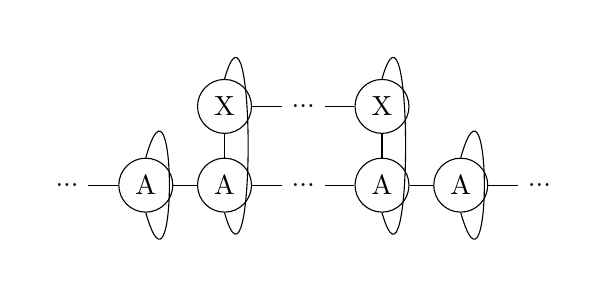
\begin{tikzpicture} [   ]
            \clip (-1.5,-1) rectangle (5.5,2);

            \node[] (N0) at (-1,0) {...};
            \node[circle, draw] (N1) at (0,0) {A};
            \node[circle, draw] (N2) at (1,0) {A};
            \node[circle, draw] (X2) at (1,1) {X};

            \node[] (N3) at (2 ,0) {...};
            \node[] (X3) at (2,1) {...};

            \node[circle, draw] (N4) at (3 ,0) {A};
            \node[circle, draw] (X4) at (3,1) {X};

            \node[circle, draw] (N5) at (4 ,0) {A};
            \node[] (N6) at (5 ,0) {...};

            \draw  (N0) -- (N1) ;

            \draw  (N1) -- (N2) ;
            \draw  (N2) -- (N3) ;
            \draw  (N3) -- (N4) ;
            \draw  (N4) -- (N5) ;
            \draw  (N5) -- (N6) ;


            \draw  (X2) -- (X3) ;
            \draw  (X3) -- (X4) ;

            \draw  (N2) -- (X2) ;
            \draw  (N4) -- (X4) ;

            \draw (X2.north)   .. controls +(0.4,1.4) and +(0.4,-1.4) .. (N2.south);
            \draw (X4.north)   .. controls +(0.4,1.4) and +(0.4,-1.4) .. (N4.south);


            \draw (N1.north)   .. controls +(0.4,1.4) and +(0.4,-1.4) .. (N1.south);
            \draw (N5.north)   ..  controls +(0.4,1.4) and +(0.4,-1.4)  .. (N5.south);
        \end{tikzpicture}
    }{
        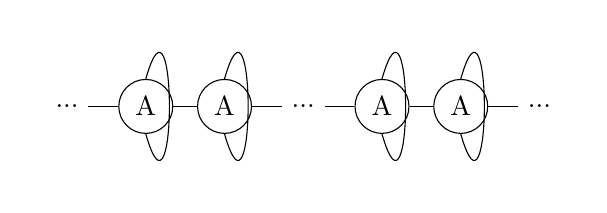
\begin{tikzpicture} [   ]

            \clip  (-1.5,-3) rectangle (5.5,-1);


            \node[] (O0) at (-1,-2) {...};
            \node[circle, draw] (O1) at (0,-2) {A};
            \node[circle, draw] (O2) at (1,-2) {A};


            \node[] (O3) at (2 ,-2) {...};
            \node[circle, draw] (O4) at (3 ,-2) {A};

            \node[circle, draw] (O5) at (4 ,-2) {A};
            \node[] (O6) at (5 ,-2) {...};

            \draw  (O0) -- (O1) ;

            \draw  (O1) -- (O2) ;
            \draw  (O2) -- (O3) ;
            \draw  (O3) -- (O4) ;
            \draw  (O4) -- (O5) ;
            \draw  (O5) -- (O6) ;


            \draw (O2.north)   .. controls +(0.4,1.4) and +(0.4,-1.4) .. (O2.south);
            \draw (O4.north)   .. controls +(0.4,1.4) and +(0.4,-1.4) .. (O4.south);


            \draw (O1.north)   .. controls +(0.4,1.4) and +(0.4,-1.4) .. (O1.south);
            \draw (O5.north)   ..  controls +(0.4,1.4) and +(0.4,-1.4)  .. (O5.south);
        \end{tikzpicture}
    }
    \label{sm:expecatation_X}
\end{equation}


In the thermodynamic limit there are an infinity number of A to the left and the right. This can be simulated by taking the left and right fixed points of the traced MPO A corresponding to the largest eigenvector $\lambda$.

\begin{equation}
    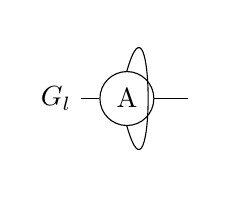
\begin{tikzpicture}[baseline={0cm-0.5*height("$=$")} , scale=0.9]
        \clip (-1.4,-1) rectangle (1,1);
        \node[] (N0) at (-1,0) {$G_l$};
        \node[] (N2) at (1,0) {};
        \node[circle, draw] (N1) at (0,0) {A};
        \draw  (N0) -- (N1) ;
        \draw  (N1) -- (N2) ;
        \draw (N1.north)   .. controls +(0.4,1.4) and +(0.4,-1.4) .. (N1.south);
    \end{tikzpicture}
    = \lambda
    \begin{tikzpicture}[baseline={0cm-0.5*height("$=$")}, scale=0.9 ]
        \clip (-.4,0.5) rectangle (1,-0.5);
        \node[] (N2) at (1,0) {};
        \node[] (N1) at (0,0) {$G_l$};
        \draw  (N1) -- (N2) ;
    \end{tikzpicture}
\end{equation}

\begin{equation}
    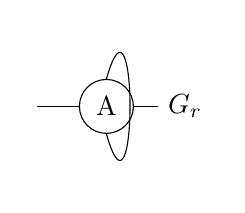
\begin{tikzpicture}[baseline={0cm-0.5*height("$=$")} ]
        \clip (-1,-1) rectangle (1.4,1);
        \node[] (N0) at (-1,0) {};
        \node[] (N2) at (1,0) {$G_r$};
        \node[circle, draw] (N1) at (0,0) {A};
        \draw  (N0) -- (N1) ;
        \draw  (N1) -- (N2) ;
        \draw (N1.north)   .. controls +(0.4,1.4) and +(0.4,-1.4) .. (N1.south);
    \end{tikzpicture}
    = \lambda
    \begin{tikzpicture}[baseline={0cm-0.5*height("$=$")} ]
        \clip (0,-0.5) rectangle (1.4,0.5);
        \node[] (N2) at (1,0) {$G_l$};
        \node[] (N1) at (0,0) {};
        \draw  (N1) -- (N2) ;
    \end{tikzpicture}
\end{equation}

Equation \cref{sm:expecatation_X} can now be easily caclulated:

\begin{equation}
    \Braket{X} = \frac{
        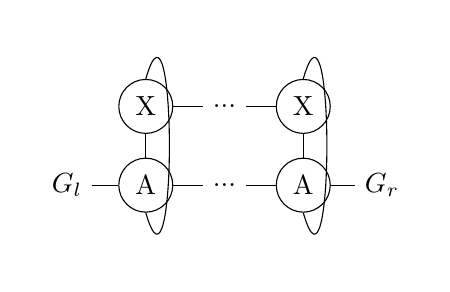
\begin{tikzpicture} [   ]
            \clip (-0.5,-1) rectangle (4.5,2);


            \node[] (N1) at (0,0) {$G_l$};
            \node[circle, draw] (N2) at (1,0) {A};
            \node[circle, draw] (X2) at (1,1) {X};

            \node[] (N3) at (2 ,0) {...};
            \node[] (X3) at (2,1) {...};

            \node[circle, draw] (N4) at (3 ,0) {A};
            \node[circle, draw] (X4) at (3,1) {X};

            \node[] (N5) at (4 ,0) {$G_r$};


            \draw  (N1) -- (N2) ;
            \draw  (N2) -- (N3) ;
            \draw  (N3) -- (N4) ;
            \draw  (N4) -- (N5) ;



            \draw  (X2) -- (X3) ;
            \draw  (X3) -- (X4) ;

            \draw  (N2) -- (X2) ;
            \draw  (N4) -- (X4) ;

            \draw (X2.north)   .. controls +(0.4,1.4) and +(0.4,-1.4) .. (N2.south);
            \draw (X4.north)   .. controls +(0.4,1.4) and +(0.4,-1.4) .. (N4.south);

        \end{tikzpicture}
    }{
        \lambda^n
        \begin{tikzpicture}[baseline={0cm-0.5*height("$=$")} ]
            \clip (-0.5,-0.5) rectangle (1.4,0.5);
            \node[] (N2) at (1,0) {$G_r$};
            \node[] (N1) at (0,0) {$G_r$};
            \draw  (N1) -- (N2) ;
        \end{tikzpicture}
    }
    \label{sm:expecatation_X_2}
\end{equation}